\documentclass[11pt]{article}
\usepackage{graphicx}
\graphicspath{ {.} }
\title{Project 1 - Markovian Queue Implementation}
\author{Harshavardhan Nalajala}
\date{October 23 2017}
\begin{document}
\maketitle
 \tableofcontents
 
 \section{Data Structures }
 \begin{itemize}
 \item Min Heap to store the requests ordered by time. Event that occurs in the most near future is stored at the root of the heap. Max heap size is dependent on the requests generated.
 In the current project, heap size is dependent on L(no. of terminals) since each terminal cannot generate another request until current request from the terminal is processed by the system.
 \item Queue to store the requests that arrived at the system but servers are busy. Max queue size is order of K(Queue size).
 \end{itemize}
 
 \section{ReadMe}
 \begin{itemize}
 \item main.c contains the main simulation program (run\textunderscore simulation API).
 \item utils.c is used to store data structures and generate exponential random variables.
 \item utils.h contains the structures and API used by main.c and implemented in utils.c
 \item input.in contains the input to be given to the program. Following is the input style.
 \begin{itemize}
 \item no. of events to be generated for each run, 'run'
 \item no. of terminals, L
 \item queue size, K
 \item no. of servers, m
 \item service time of each server, 'mu'
 \end{itemize}
 \item plotter.py python script to generate the graphs of output obtained from simulation.
 \item avg\textunderscore output file contains the output as lambda, expected no., theoritical expected no., expected time, theoritical expected time, blocking probability, theoritical blocking probability, utilization of the system, theoritical utilization of the system.
 \item q\textunderscore simulator executable to be run.
 \item run\textunderscore script shell script file to build and run the simulation. Use following method to run the simulation.
 \begin{itemize}
 \item modify input.in as per above instructions
 \item ./run\textunderscore script.sh 
 \end{itemize}
 \end{itemize}
 \section{Dependencies}
 \begin{itemize}
 \item gcc compiler
 \item python3. For python2 or 2.7, run\textunderscore script needs to be modified to enable python2. 
 \end{itemize}
 \section{OUTPUTS}
 \subsection{L1, K4, M2, U3}
 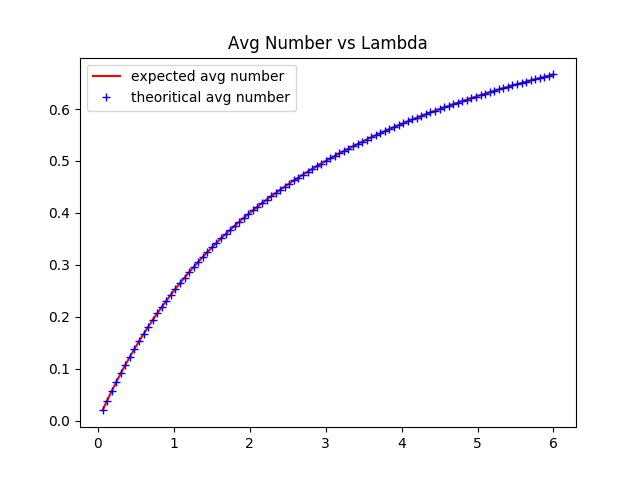
\includegraphics{ExpectedNumber_L1_K4_M2_U3}
  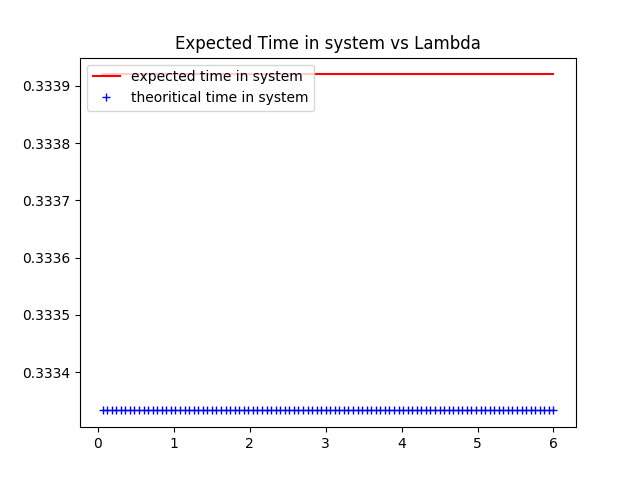
\includegraphics{ExpectedTime_L1_K4_M2_U3}
 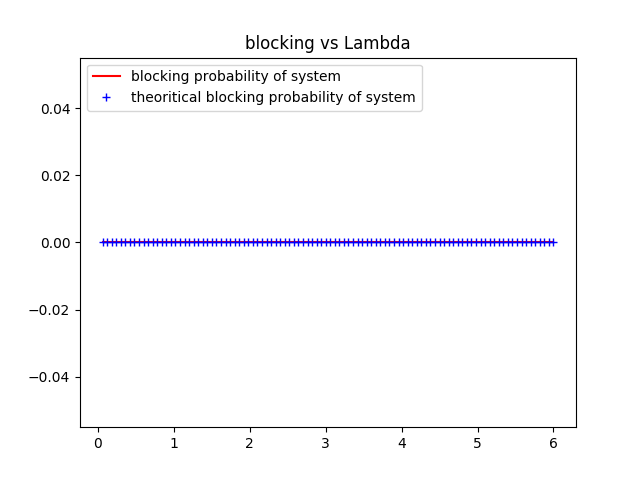
\includegraphics{BlockingProbability_L1_K4_M2_U3}
 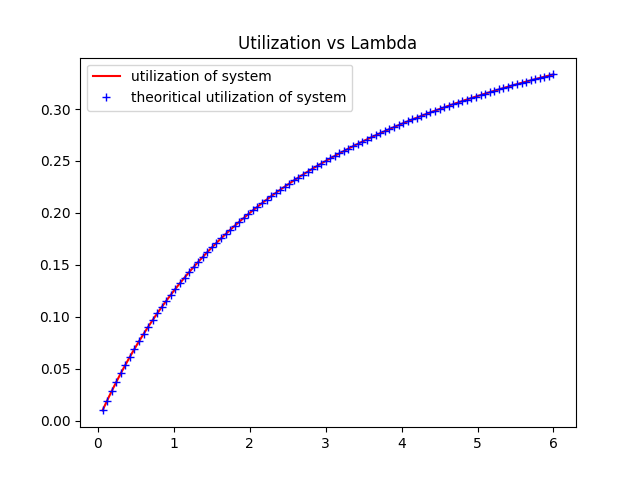
\includegraphics{Utilization_L1_K4_M2_U3}

\subsection{L10, K4, M2, U3}
 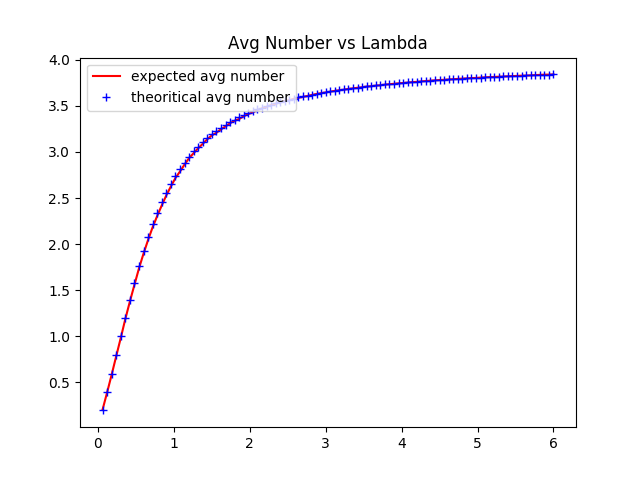
\includegraphics{ExpectedNumber_L10_K4_M2_U3}
  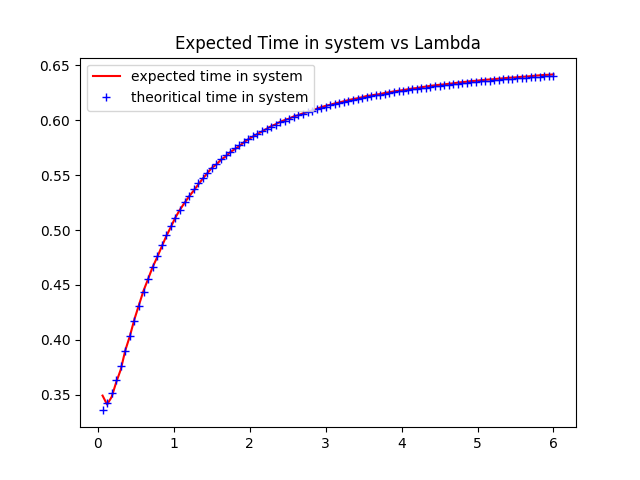
\includegraphics{ExpectedTime_L10_K4_M2_U3}
 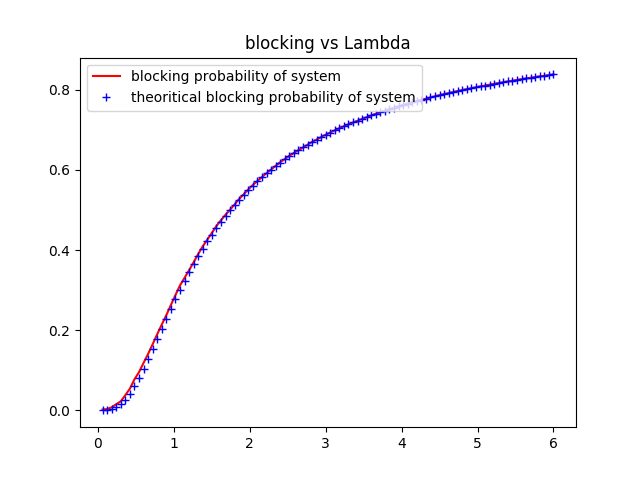
\includegraphics{BlockingProbability_L10_K4_M2_U3}
 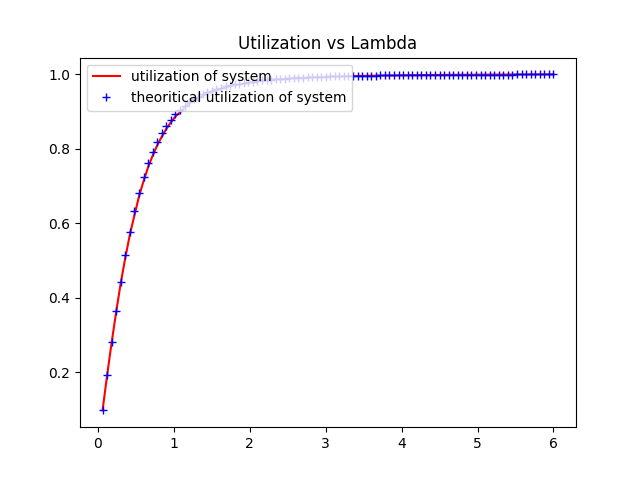
\includegraphics{Utilization_L10_K4_M2_U3}
 
 \subsection{L1000, K4, M2, U3}
 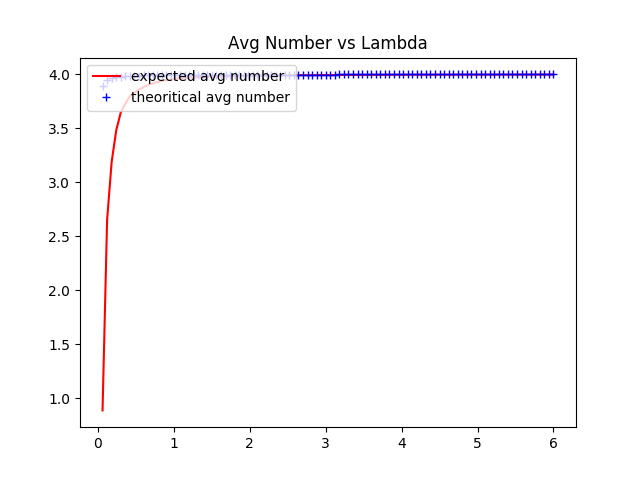
\includegraphics{ExpectedNumber_L1000_K4_M2_U3}
  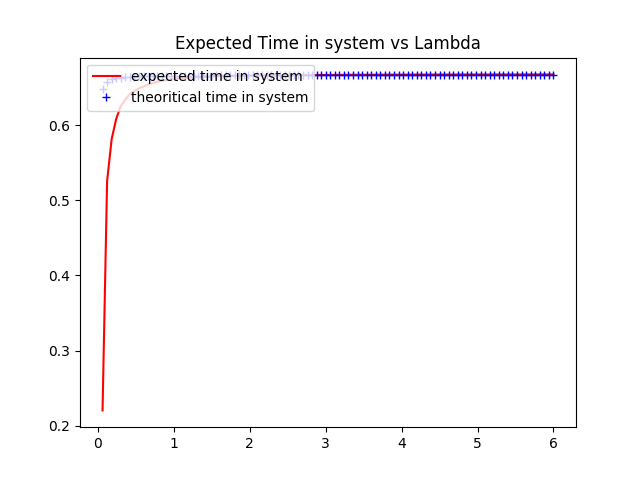
\includegraphics{ExpectedTime_L1000_K4_M2_U3}
 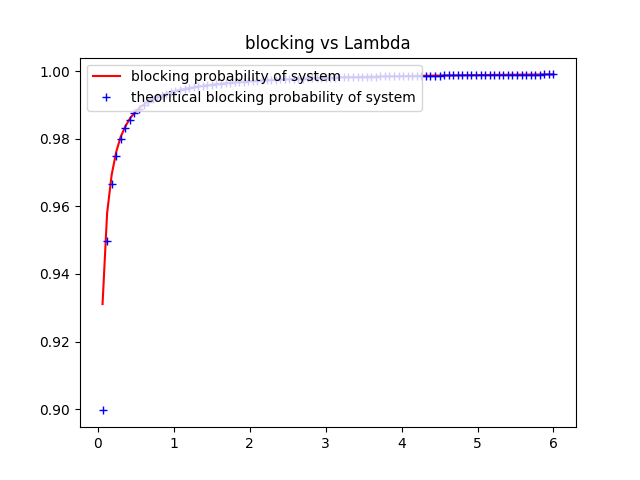
\includegraphics{BlockingProbability_L1000_K4_M2_U3}
 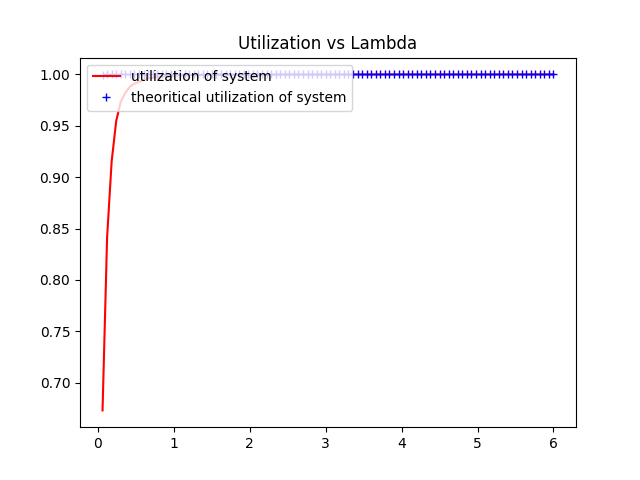
\includegraphics{Utilization_L1000_K4_M2_U3}
 
 \subsection{L10, K4, M4, U3}
 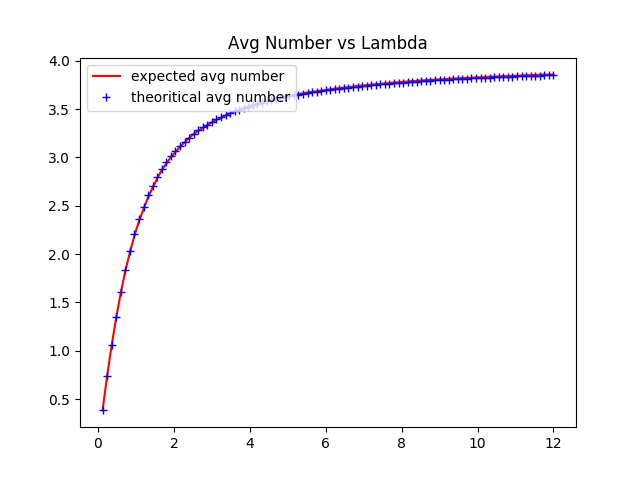
\includegraphics{ExpectedNumber_L10_K4_M4_U3}
  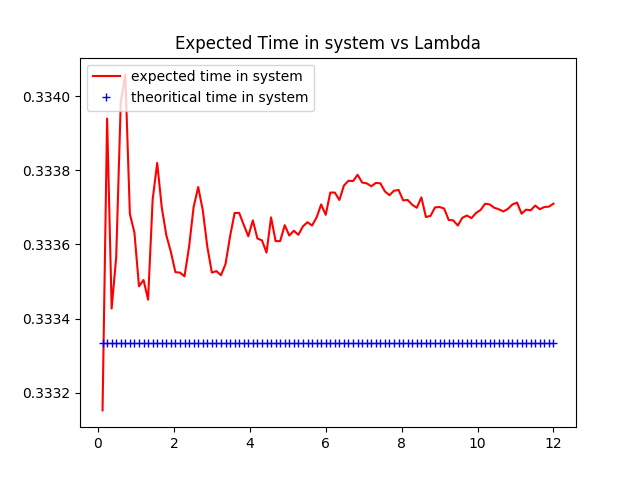
\includegraphics{ExpectedTime_L10_K4_M4_U3}
 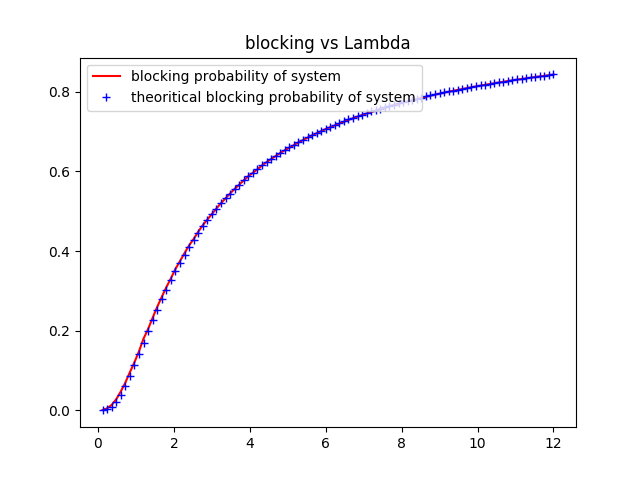
\includegraphics{BlockingProbability_L10_K4_M4_U3}
 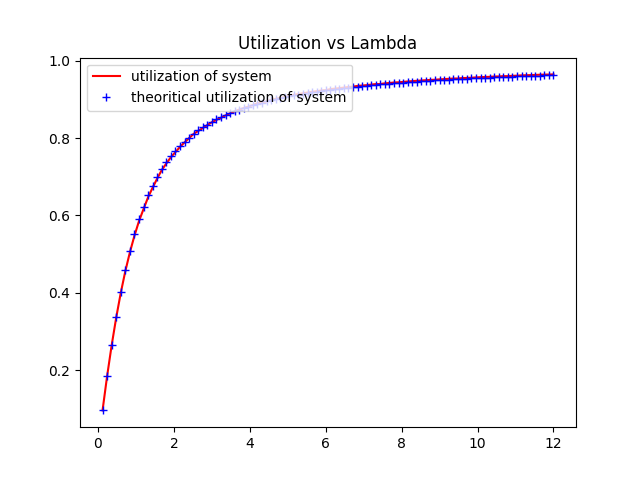
\includegraphics{Utilization_L10_K4_M4_U3}
 
 \section{Limitations}
 Heap size is set to 1000 in utils.h. As long as number of events at any point of time is not more than 1000, simulator is fine. However we can modify the value and run the script again. Script builds the code and runs the simulation again.
\end{document}